\documentclass[tikz]{standalone}

\usetikzlibrary{shapes}
\usetikzlibrary{calc} 

\usetikzlibrary{decorations.pathreplacing}
\usetikzlibrary{decorations.markings}
\usetikzlibrary{decorations.pathmorphing}
\usetikzlibrary{decorations.text}

\usepackage{mathtools}
\providecommand\enpos[2]{\underset{\footnotesize\mathbf{\mathclap{\left\lfloor#1,#2\right\rceil}}}{N}}
% This bascially automates a \newcommand{<name>}{} to ensure
% that a command with the given <name> does not already exist
\providecommand*{\pgfmathsetnewmacro}[2]{%
    \newcommand*{#1}{}% Error if already defined
    \pgfmathsetmacro{#1}{#2}%
}%

\begin{document}

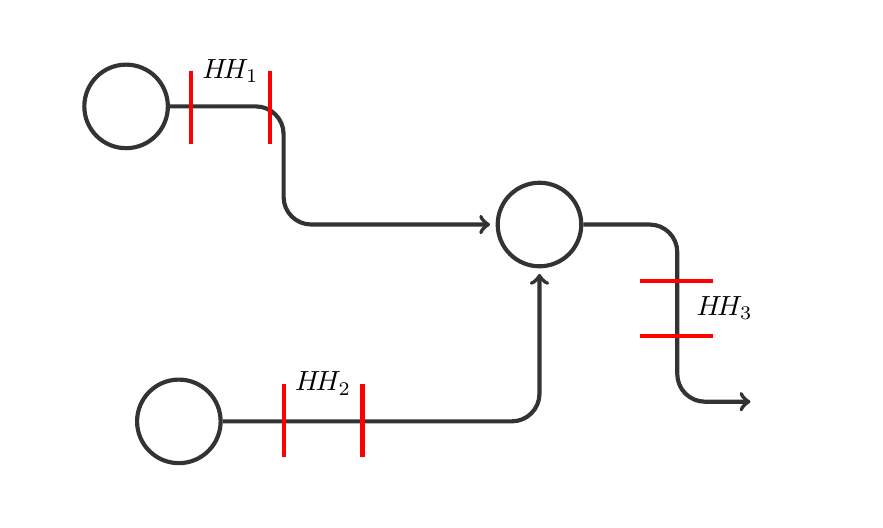
\begin{tikzpicture}[%
        scale = 1,
        draw = black!80,
        fill = white,
        line width = 1.5pt,
        rounded corners = 10pt,
        shorten >=2pt,
        % decoration={random steps, amplitude = 0.25cm, segment length=0.8cm},
        % smooth
        ]

\useasboundingbox[] (-5.25,-3) rectangle (5.25,3);
% \draw (-5,-3) grid (5,3);


\node (N1) [circle, draw, fill = white] at (-4,2) 
    {\large \phantom{$\enpos{1}{0}$}%
    };
\node (N2) [circle, draw, fill = white] at (-3.33,-2)
    {\large \phantom{$\enpos{1}{1}$}%
    };


\node (N3) [circle, draw, fill = white] at (1.25,0.5)
    {\large \phantom{$\enpos{2}{0}$}%
    };


\draw[->,decorate] (N1) -- +(0:2) |- (N3);
\draw[->,decorate] (N2) -| (N3);

\draw[->,decorate] (N3) -| (3,-1.75) -- +(0:1);


\node (a) [fill] at ($(N1)+(0:2)!0.9!(N3)$) {$H\!H_1$};
\foreach \SIGN in {+,-}{
    \path (a) -- +(90\SIGN90:0.5cm) coordinate (a\SIGN);
    \draw[red] (a\SIGN) -- +(270:1);
    }


\node (b) [fill] at ($(N2)!0.4!(N3)+(270:0.52)$) {$H\!H_2$};
\foreach \SIGN in {+,-}{
    \path (b) -- +(90\SIGN90:0.5cm) coordinate (b\SIGN);
    \draw[red] (b\SIGN) -- +(270:1);
    }

\node (c) [fill, anchor = west, xshift = -0.13cm] at ($(N3)!0.85!(4,-0.75)$) {$\mathclap{H\!H_3}$};
\foreach \SIGN in {+,-}{
    \path (c.west) -- +(\SIGN90:0.35cm) coordinate (c\SIGN);
    \draw[red] (c\SIGN) -- +(180:1);
    }


\end{tikzpicture}

\end{document}